%!TEX root = PMP_ClockPendulumAnalyzer.tex
\subsection*{Sprint 1}
Die Planung und der Abschluss von Sprint 1 ist in diesem Kapitel aufgeführt.
\subsubsection*{Planung}
Die Planung der Sprints wurde mit dem Programm Taiga.io durchgeführt. Unten ist ein Screenshot zu Beginn von Sprint 1.
    \begin{figure}[H]
        \centering
        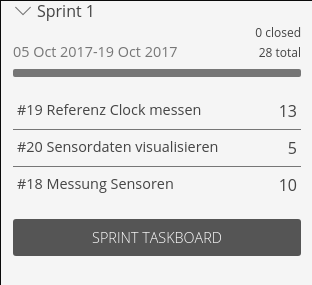
\includegraphics[width=.5\textwidth]{sprint1_plan.png}
        \caption{Sprintplanung für Sprint 1}
    \end{figure}
\subsubsection*{Sprintreview}
    Sprint 1 wurde mit zufrieden stellenden Ergebnissen aus verschiedenen einzelnen Tasks beendet. Die involvierten User Stories wurden mit untenstehender Begründung in den nächsten Sprint verschoben.
    \begin{table}[H]
        \centering
        \begin{tabular}{lccp{7cm}}
            \textbf{User Story} &  \textbf{Status} & \textbf{Sprintziel}& \textbf{Begründung}\\\toprule[2pt]
            \#19 Referenz Clock messen & teilweise erledigt & Verschoben & Auf Grund von Wartezeiten\\
            \#20 Sensordaten visualisieren & teilweise erledigt & Verschoben & einzelne Tasks konnten wegen fehlendem Werkzeug nicht komplettiert werden\\
            \#18 Messung Sensoren & teilweise erledigt & Verschoben & Tasks konnten aufgrund Abwesenheit nicht vervollständigt werden\\
        \end{tabular}
        \caption{Status der User Stories aus Sprint 1}
    \end{table}